\documentclass[11pt]{exam}
\usepackage[utf8]{inputenc}
\usepackage{hyperref}
\usepackage{graphicx}

\title{Reglas de Asociación en Weka}
\author{Laura Rodríguez Navas \\ rodrigueznavas@posgrado.uimp.es}
\date{\today}

\pagestyle{plain}

\begin{document}

\maketitle

En esta práctica se realiza un estudio acerca de los datos del hundimiento del Titanic a través de la herramienta \href{https://www.cs.waikato.ac.nz/ml/weka/}{Weka}. Los datos se encuentran en la dirección \url{http://www.hakank.org/weka/titanic.arff} y corresponden a las características de los 2201 pasajeros del Titanic. Estos datos son reales y se han obtenido de \textit{"Report on the Loss of the 'Titanic' (S.S.)" (1990), British Board of Trade Inquiry Report\_(reprint), Gloucester, UK: Allan Sutton Publishing}.

\vspace{3mm}

Para realizar esta práctica, se debe cargar el dataset Titanic que se ha descargado anteriormente y contestar a las siguientes preguntas:

\begin{questions}

% Pregunta 1
{\question Cuando ejecutamos el algoritmo Apriori de Weka, podemos utilizar diferentes umbrales de soporte. Dependiendo de qué umbrales de soporte pongamos, nos saldrán más o menos itemsets. Como resultado, Weka nos proporciona un conjunto de ítems L(1)... L(4) cuyos números van variando conforme cambiamos el umbral de soporte. Responde a las siguientes preguntas, utilizando capturas de pantalla y explicando los resultados de manera clara y concisa:}

\begin{parts}
\part ¿Qué representan cada uno de estos conjuntos de ítems? 

\begin{figure}[h]
\centering
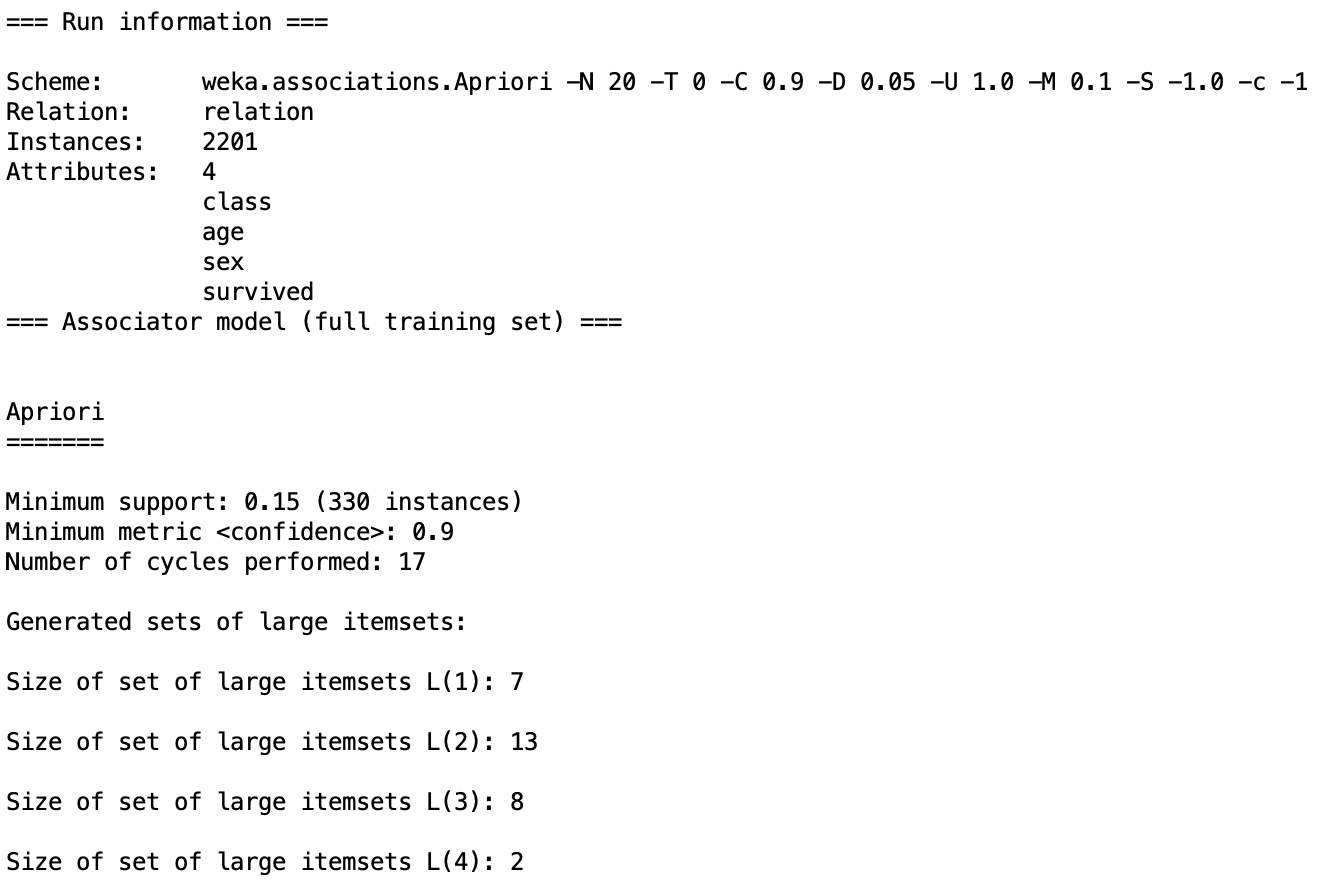
\includegraphics[scale=0.6]{Captura_1_1.png}
\end{figure}

\begin{enumerate}
\item El conjunto de ítems L(1) representa el número de conjuntos de ítems de tamaño 1. Que en este caso es 7.
\item El conjunto de ítems L(2) representa el número de conjuntos de ítems de tamaño 2. Que en este caso es 13.
\item El conjunto de ítems L(3) representa el número de conjuntos de ítems de tamaño 3. Que en este caso es 8.
\item El conjunto de ítems L(4) representa el número de conjuntos de ítems de tamaño 4. Que en este caso es 2.
\end{enumerate}	

\part ¿Puede existir L(0)? Explica porqué.

No. El conjunto de ítems L(0) representaría el número de conjuntos de ítems de tamaño 0, es decir, el conjunto de ítems vacío, que no es válido como conjunto de ítems.

\part ¿Puede existir L(5)? Explica porqué.

No. Porqué el dataset de Titanic solo contiene cuatro atributos diferentes.

\begin{center}
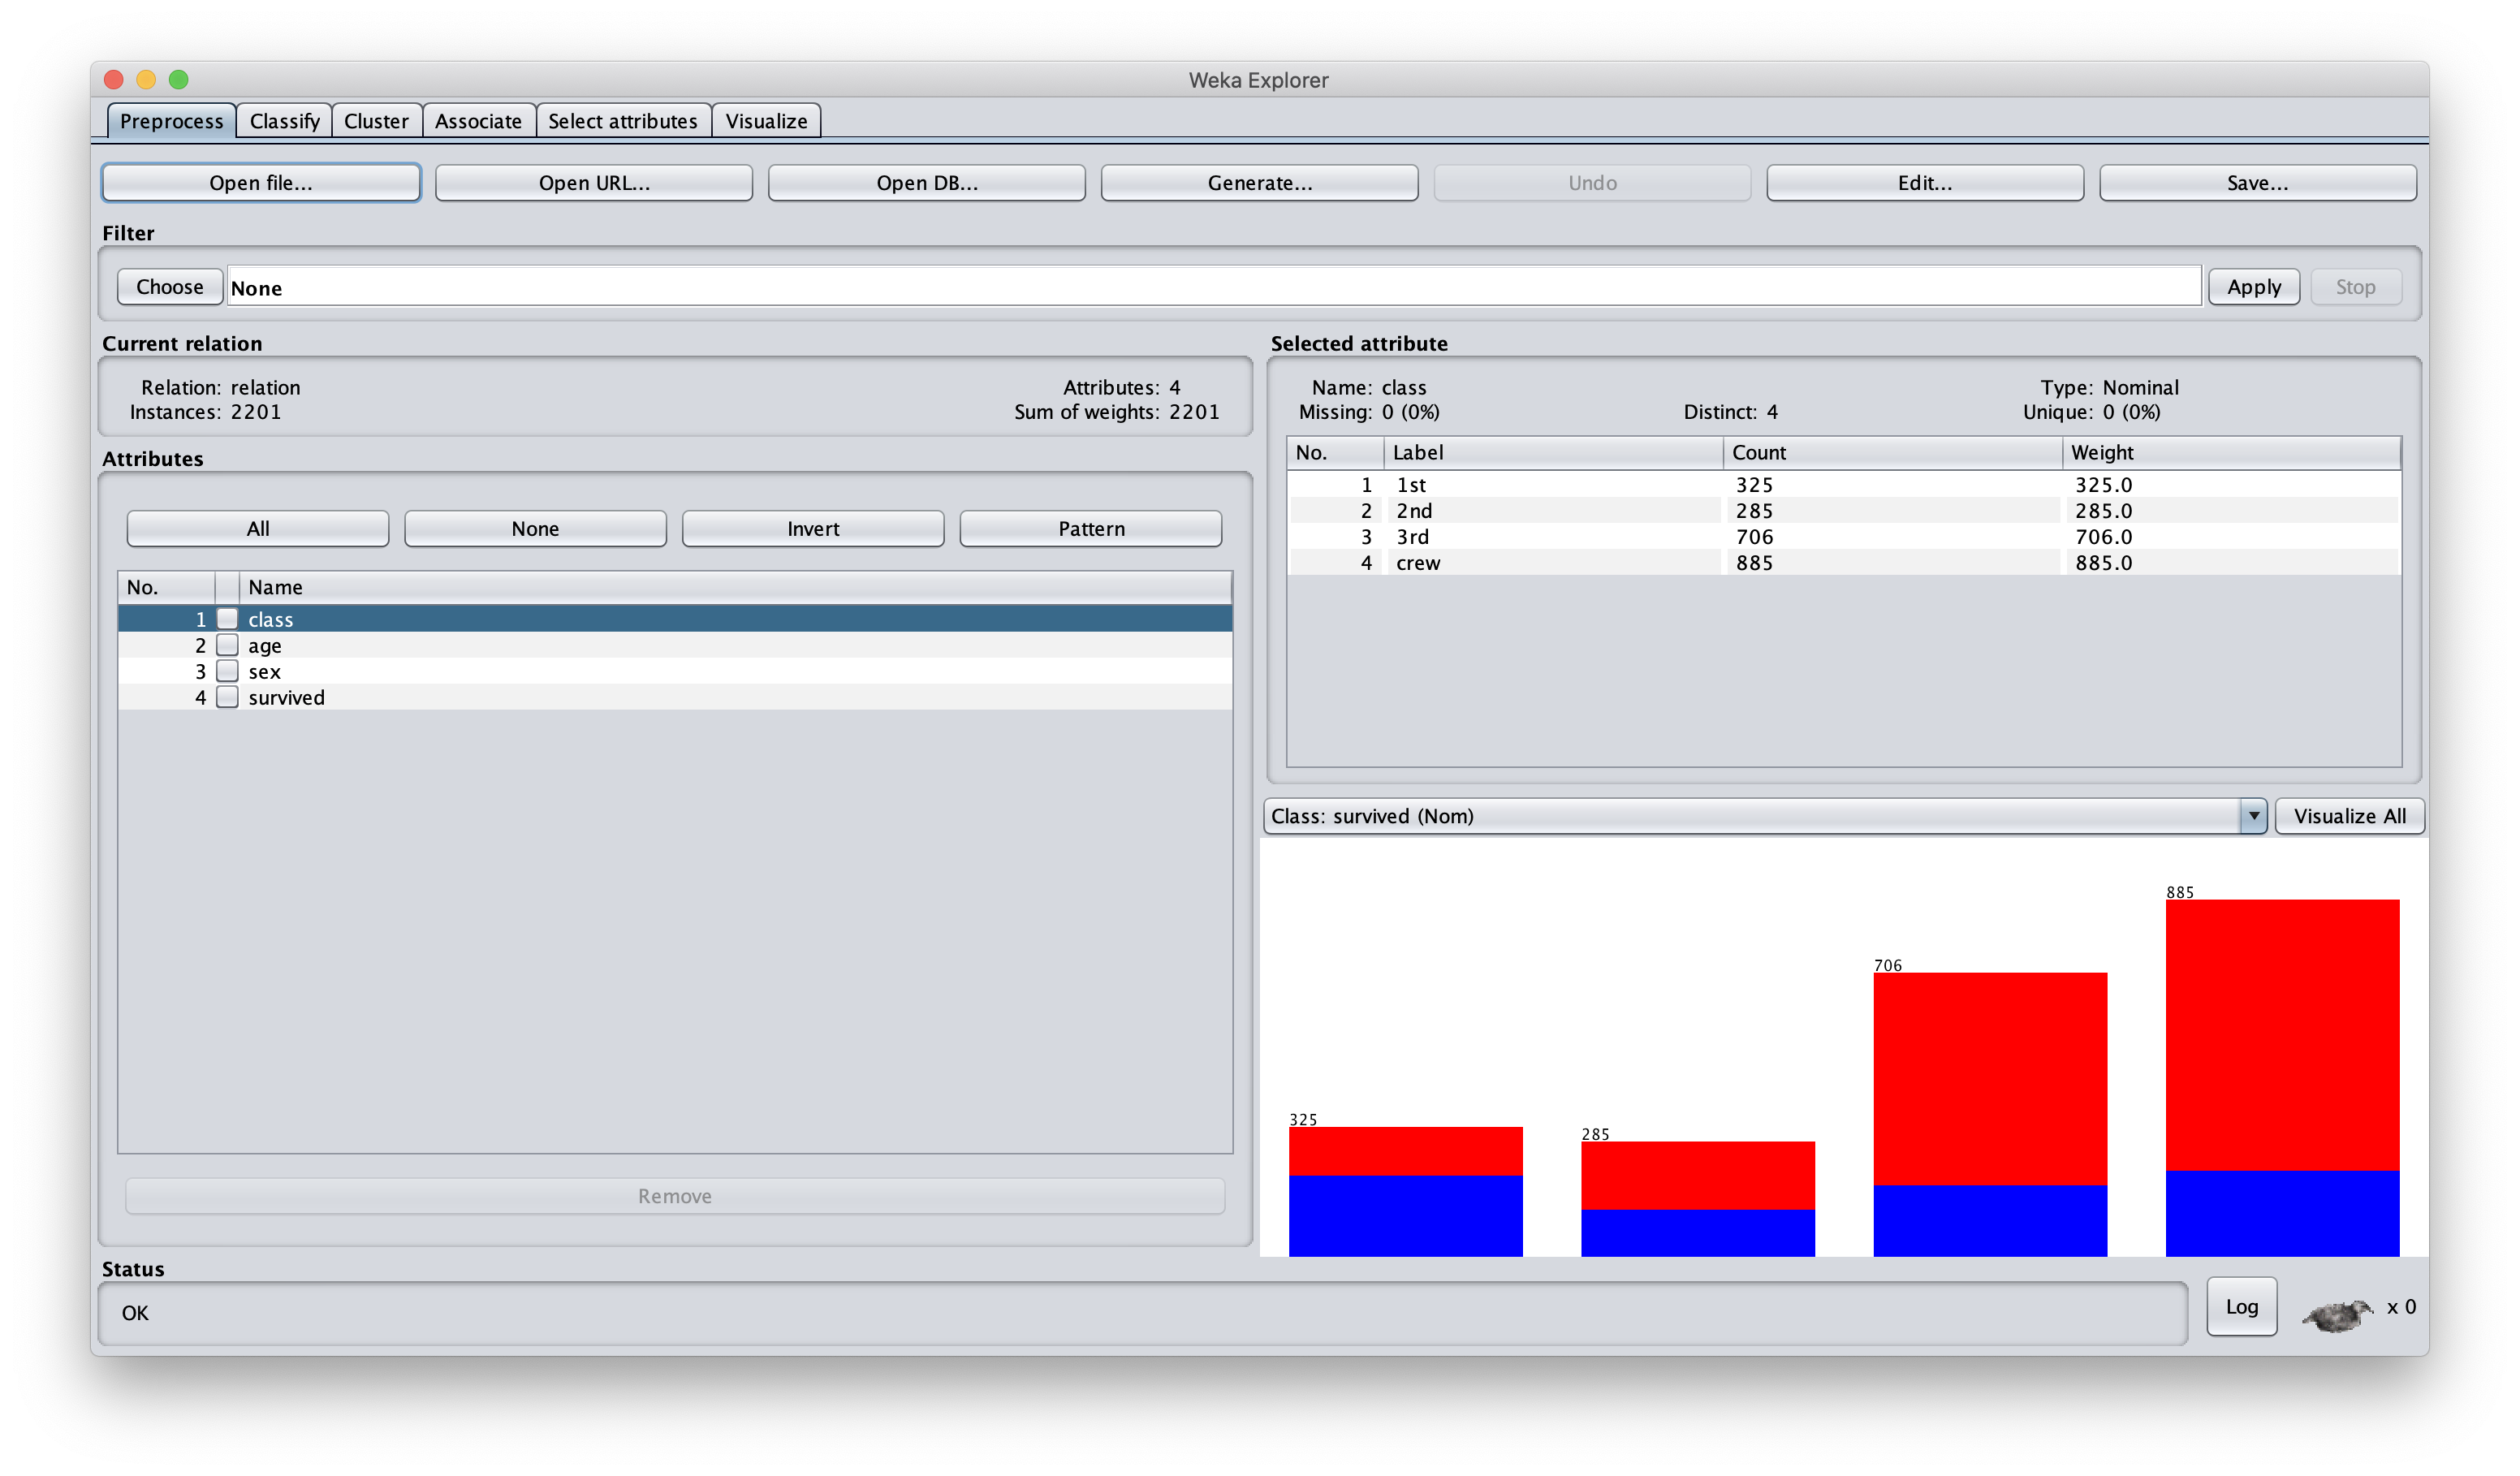
\includegraphics[scale=0.25]{Captura_1_2.png}
\end{center}

\part ¿Puede L(1) tomar un valor mayor que 10? Explica de manera teórica que eso no es posible y compruébalo experimentalmente.

No. El conjunto de ítems de tamaño 1, como máximo, tendrá un valor de 9.  Ya que el conjunto como máximo puede formarse por los diferentes valores que puede tomar cada atributo del dataset. En este caso, el dataset de Titanic, contiene 9 valores diferentes, como vemos a continuación:

\begin{itemize}
	\item Class ("1st", "2nd", "3rd", "Crew")
	\item Age {"Adult", "Child"}
	\item Sex {"Male", "Female"}
	\item Survived {"Yes", "No"}
\end{itemize}

El algoritmo Apriori siempre comienza obteniendo los itemsets más fecuentes de tamaño 1. Donde, el número de ocurrencias de estos es 1. Para comprobarlo experimentalmente, el umbral de confianza debe ser igual a 1.

\begin{figure}[h]
	\centering
	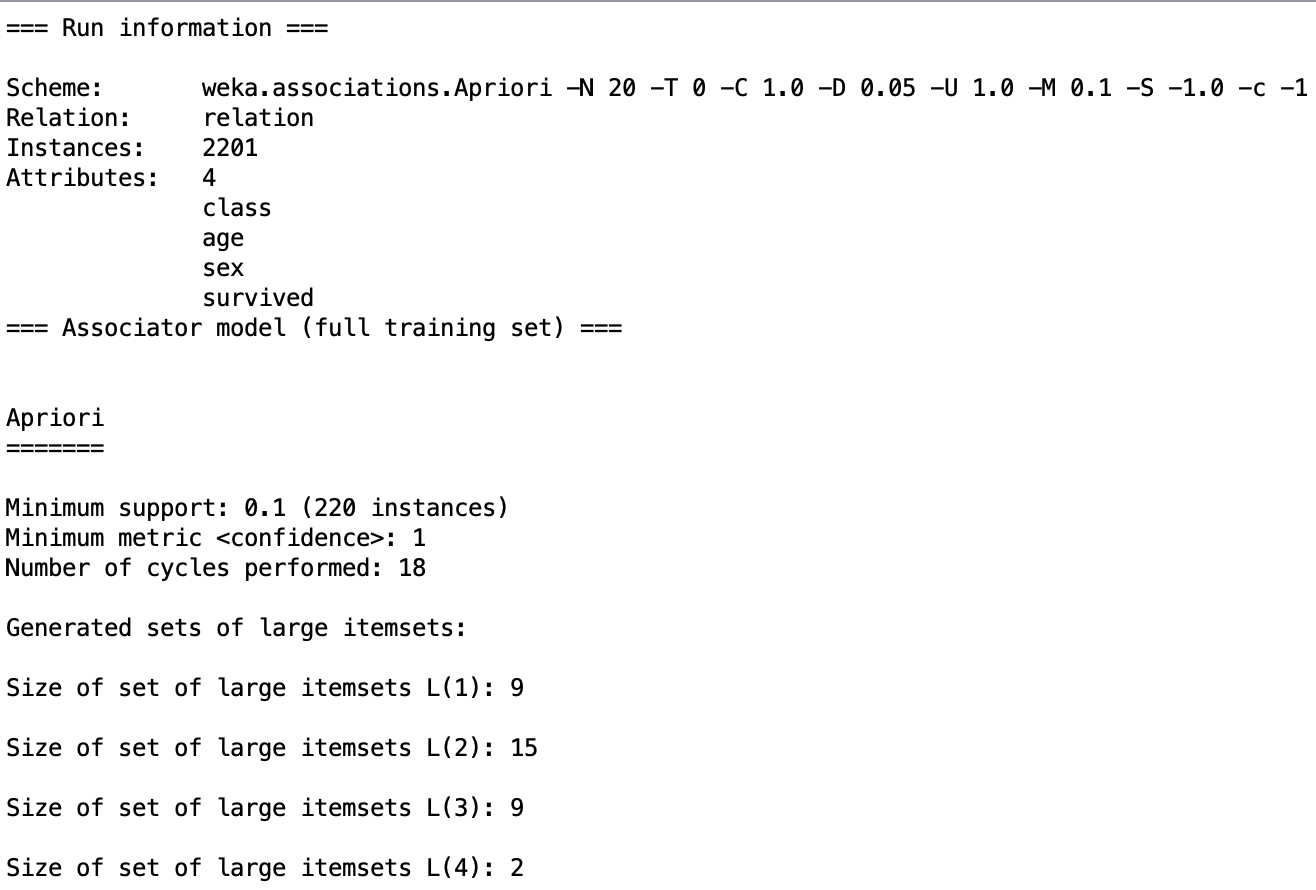
\includegraphics[scale=0.6]{Captura_1_3.png}
\end{figure}

\end{parts}

% Pregunta 2
{\question Además de los valores de soporte, el algoritmo Apriori de Weka nos permite utilizar diferentes umbrales de soporte y confianza. Responde a las siguientes preguntas, utilizando capturas de pantalla y explicando los resultados de manera clara y concisa:}

\begin{parts}
\part ¿Es posible que una regla tenga un valor de soporte inferior a su confianza? Explica porqué y demuéstralo experimentalmente.

Sí.

\begin{figure}[h]
	\centering
	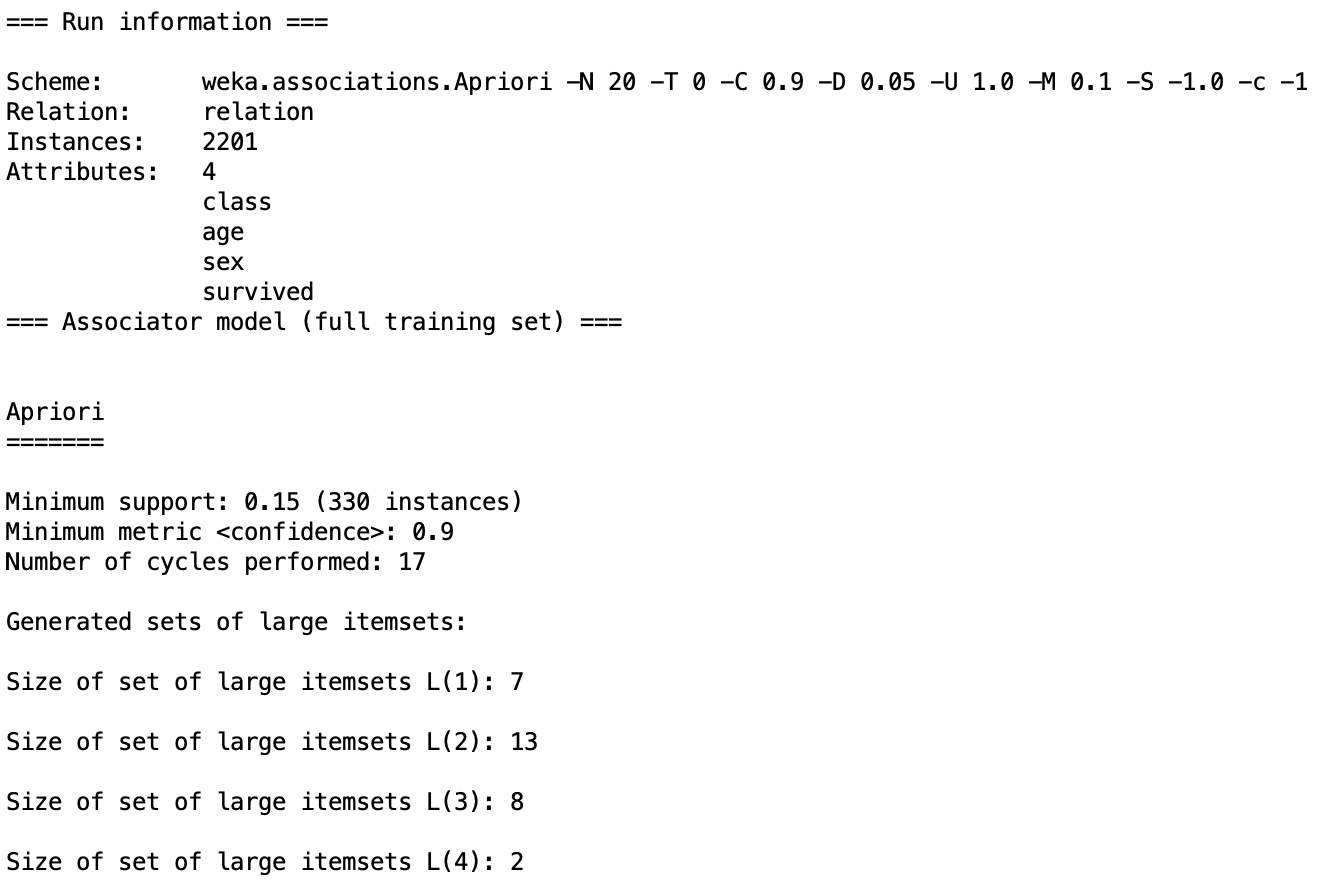
\includegraphics[scale=0.6]{Captura_1_1.png}
\end{figure}

\part ¿Es posible que una regla tenga un valor de confianza inferior a su suporte? Explica porqué y demuéstralo experimentalmente.

Sí.

\begin{figure}[h]
	\centering
	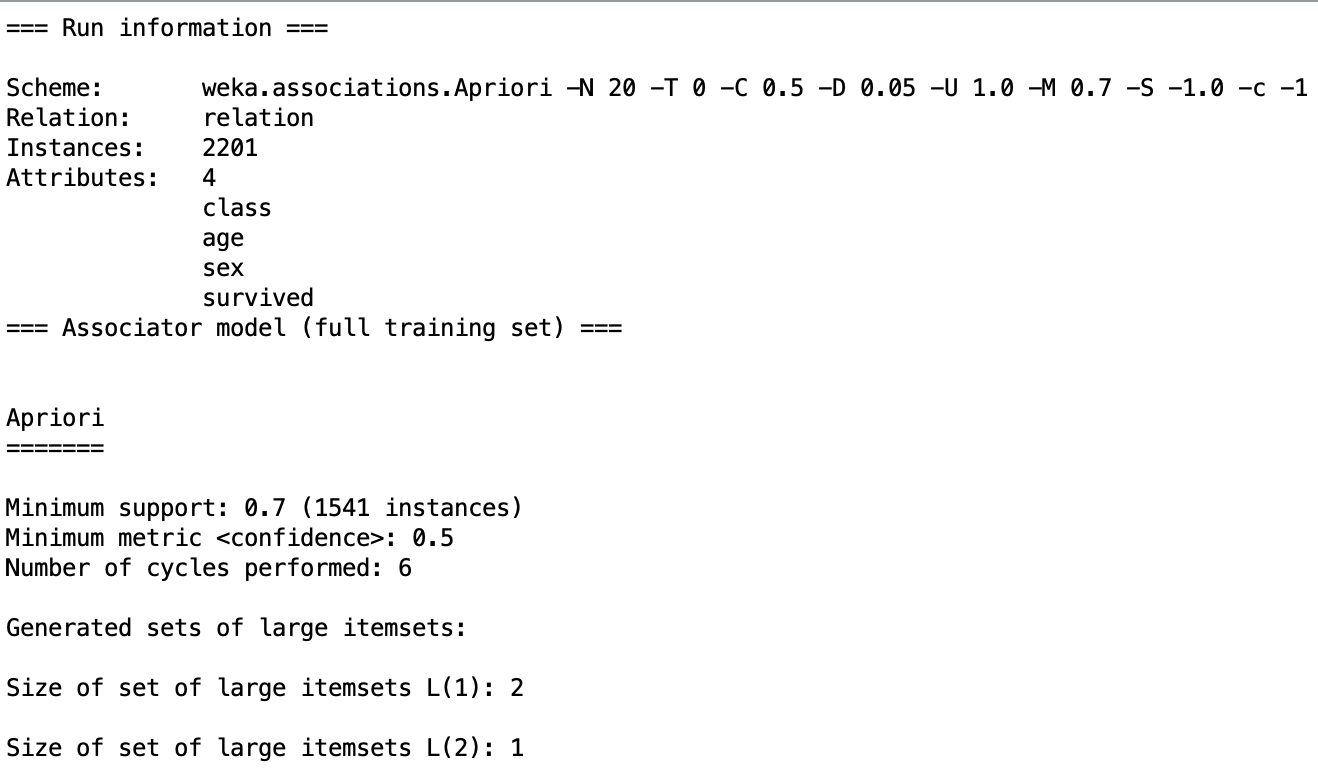
\includegraphics[scale=0.6]{Captura_1_4.png}
\end{figure}


\part La variación del umbral de confianza (dado un umbral fijo de soporte) no afecta a los 	conjuntos L(1)... L(4). ¿Por qué?
\end{parts}



% Pregunta 3
{\question Usaremos ahora, 0.75 como valor mínimo de soporte y de confianza 0.00. Comprobamos que obtenemos dos reglas de asociación, sin embargo, L(2) es 1. ¿Qué quiere decir esto? ¿A qué corresponde L(2)? ¿Qué itemset representa?}

\begin{figure}[h]
\centering
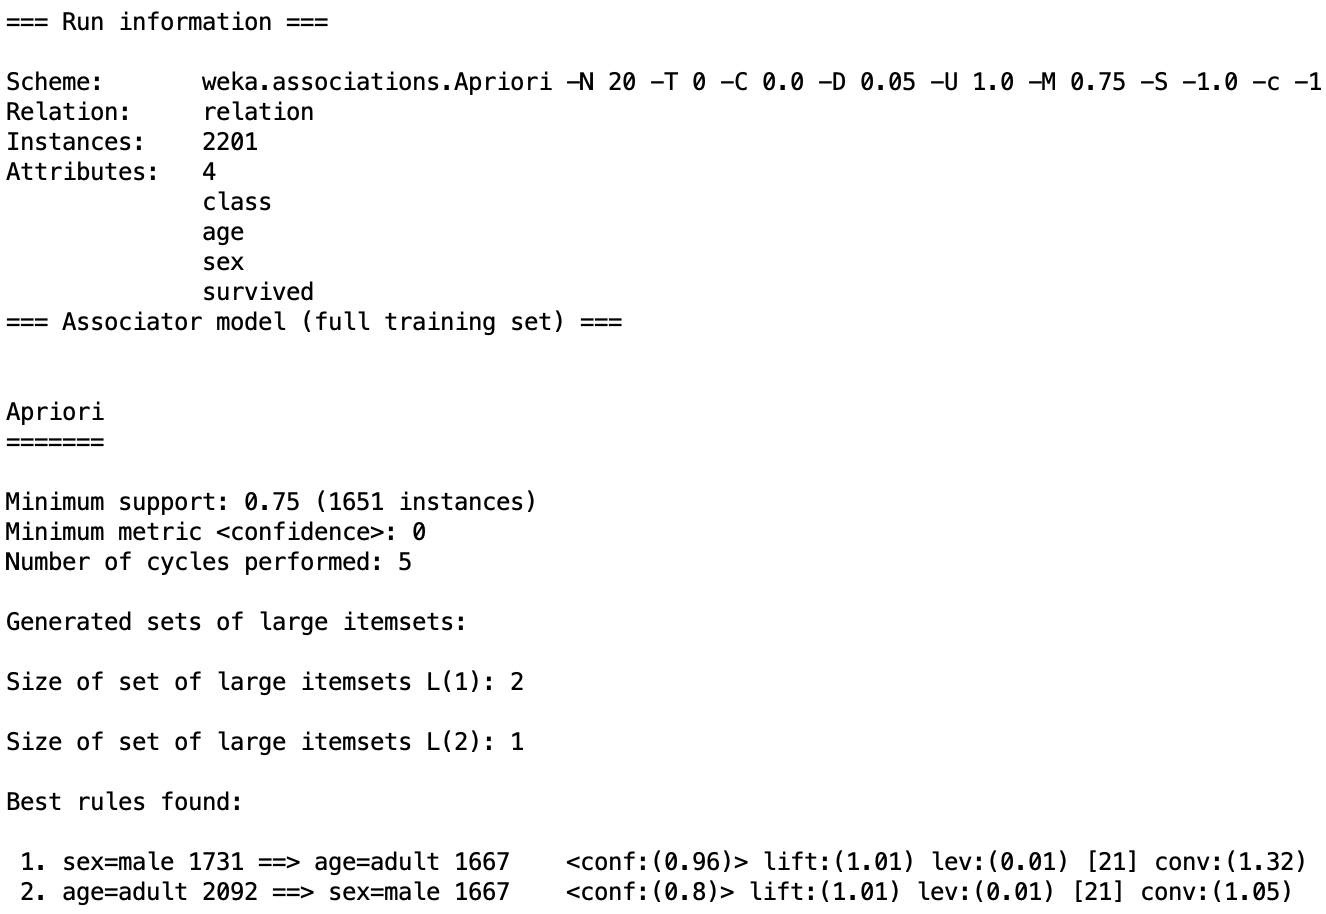
\includegraphics[scale=0.6]{Captura_1_5.png}
\end{figure}

% Pregunta 4
{\question Analiza el conjunto de reglas que salen al aplicar diferentes umbrales de soporte y confianza. Coge una regla, la que veas más interesante, y coméntala. Explica sus valores de métricas y qué representan, y el significado de la regla, es decir, el conocimiento que te aporta dicha regla.}

\end{questions}

\end{document}
